\chapter{Primjena algoritamskih paradigmi na probleme iz aritmetike}

% https://www.geeksforgeeks.org/dynamic-programming/

U ovoj glavi se bavimo rješavanjem nekih interesantnih problemi iz
aritmetike primijenjujući algoritamske paradigme koje smo obradili u prethodnoj glavi.

\section{Eratostenovo sito}

\begin{definition}
 	Broj $n \in \mathbb{N}$ je \textit{prost} akko je djeljiv isključivo sa 1 i sa samim sobom. 
\end{definition}

Npr. lista prvih 5 prostih brojeva se: 2, 3, 5, 7, i 11. Broj 6 nije prost, jer je djeljiv (pored 1 i 6) sa 2 i sa 3. 

Postavimo sljedeći zadatak. \emph{
Ispitati koliko se prostih brojeva može pronaći,
u nekom razumnom vremenu, među prvih ${N}$ prirodnih brojeva.} \\ 


Paradigmom brutalne sile, ovo bi se moglo riješiti sljedećim rezonovanjem: ispitajmo svaki od (prirodnih) brojeva u intervalu od $2$ do ${N}$ da li je prost ili ne, sljedećom jednostavnom procedurom:

\begin{minted}{python}
     
     def prost(n):
       
       for i in range(2, n):
           if n % i == 0:
              return false
       return True
\end{minted}
Kompleksnost ove procedure je $O(n)=O(N)$ i nju pozivamo $N-1$ puta. Dalje, kompleksnost ovog algoritma bi bila $O(N^2)$. Možemo  li bolje od ovoga? \\

 Iskoristimo ideju da se za neki prost broj $p$, niti jedan od brojeva $k\cdot p, k = 1, \ldots \lceil N/ p \rceil$ nije prost, osim za $k=1$. Dakle, ove brojeve možemo direktno profiltirati iz skupa $\{2, \ldots, N\}$. Zatim, isto se uradi  i za naredni prost broj $p' >p$ u nizu preostalih brojeva, i tako progresivno, sve dok ne dođemo do posljednjeg broja $N$. Dakle, u svakoj iteraciji algoritma, kroz ``sito'' prolaze (filtriraju se) brojevi koji nisu prosti, izvršavajući   provjeru da li je razmatrani broj prost ili ne u konstantnom vremenu. Brojevi koji preostanu u ``situ'' su upravo svi prosti brojevi koji su manji (ili jednaki) $N$.

Implementacija algoritma je data narednim k\^odom. 

\begin{minted}{python}
	def sieve(N):
	   
	   sieve = [True] * (N+1)
	   sieve[0] = sieve [1] = False
	   
	   p = 2
	   while p <= N:
	       
	       if  sieve[p]:
	        
	           index = 2 * p
	           while index <= N:
	               sieve[index] = False
	               index += p
	           
	        p = p + 1
	   
	   for i in range(N+1):
	       if sieve[i]: #broj je prost
	          print(i)
       #poziv funkcije:
       N = 1000
       sieve(N)
\end{minted}  
\textit{Kompleksnost algoritma}.  Može se pokazati da je kompleksnost prethodnog algoritma jednaka $O(N \log\log N )$. 


Demonstrirajmo   prvih nekoliko iteracija ovog algoritma u tabelarnom zapisu, za $N=50.$ 

U početnoj iteraciji, inicira se niz (tabela) brojeva gdje su svi brojevi označeni kao prosti (na poziciji koja odgovara broju se čuva vrijednost \emph{True}).

%\begin{figure}[H]
%	 \centering
%	 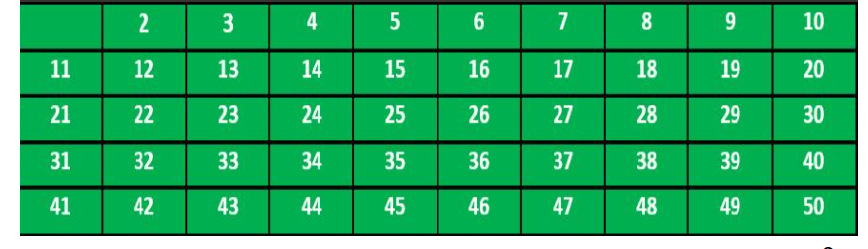
\includegraphics[width=340pt,height=120pt]{slike/sieve-it-0.png}
%\end{figure}

\begin{table}[H]
	\centering
	\begin{tabular}{|c|c|c|c|c|c|c|c|c|c|c} \hline
       & 2 & 3 & 4 & 5 & 6 & 7 & 8 & 9 & 10 \\ \hline
    11 & 12 & 13 & 14 & 15 & 16 & 17 & 18 & 19 & 20 \\ \hline
    21 & 22 & 23 & 24 & 25 & 26 & 27 & 28 & 29 & 30 \\ \hline
    31 & 32 & 33 & 34 & 35 & 36 & 37 & 38 & 39 & 40 \\ \hline
    41 & 42 & 43 & 44 & 45 & 46 & 47 & 48 & 49 & 50 \\ \hline     
	\end{tabular}
    \caption{Inicijalizacija.} \label{eratosten-sieve-it-0}
\end{table}


Dalje, u prvoj iteraciji, nalazimo se na poziciji 2, gdje elemente na pozicijama $2 \cdot k, k=2, \ldots, 50$ eliminišemo kroz sito (kao oni koji nisu prosti, dodijeljujući im vrijednost \emph{False}). Vizuelno, preostali brojevi za ispitivanje su oni neoznačeni:


%\begin{figure}[H]
%	\centering
%	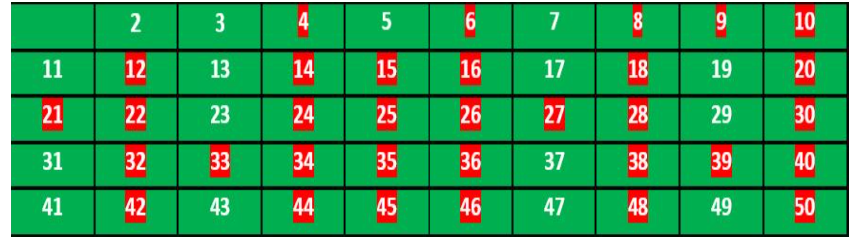
\includegraphics[width=340pt,height=120pt]{slike/sieve-it-1.png}
%\end{figure}

\begin{table}[H]
	\centering
	\begin{tabular}{|c|c|c|c|c|c|c|c|c|c|c} \hline
		& 2 & 3 & \cellcolor{red!30}  4 & 5 & \cellcolor{red!30} 6 & 7 & \cellcolor{red!30} 8 & 9 & \cellcolor{red!30} 10 \\ \hline
		11 &\cellcolor{red!30}  12 & 13 & \cellcolor{red!30} 14 & 15 & \cellcolor{red!30} 16 & 17 & \cellcolor{red!30} \cellcolor{red!30} 18 & 19 & \cellcolor{red!30} \cellcolor{red!30} 20 \\ \hline
		21 & \cellcolor{red!30} 22 & 23 & \cellcolor{red!30} 24 & 25 & \cellcolor{red!30} 26 & 27 &\cellcolor{red!30}  28 & 29 & \cellcolor{red!30} \cellcolor{red!30} 30 \\ \hline
		31 & \cellcolor{red!30} 32 & 33 & \cellcolor{red!30} 34 & 35 & \cellcolor{red!30} 36 & 37 & \cellcolor{red!30} 38 & 39 & \cellcolor{red!30} 40 \\ \hline
		41 & \cellcolor{red!30} 42 & 43 & \cellcolor{red!30} 44 & 45 & \cellcolor{red!30} 46 & 47 &\cellcolor{red!30}  48 & 49 &\cellcolor{red!30}  50 \\ \hline     
	\end{tabular}
        \caption{Eratostenovo sito: iteracija 1.} \label{eratosten-sieve-it-1}
\end{table}



Dalje, u drugoj iteraciji, prelazimo na poziciju 3. Kako je ona označena sa \emph{True} (prost broj), elemente na pozicijama $3\cdot k, k=2, \ldots, 16$ eliminišemo kroz sito (jer nisu prosti). Prelostali brojevi za ispitivanje su oni neoznačeni u narednoj tabeli. 

%\begin{figure}[H]
%	\centering
%	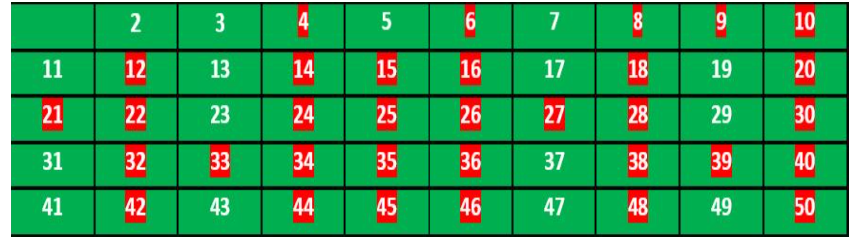
\includegraphics[width=340pt,height=120pt]{slike/sieve-it-1.png}
%\end{figure}

\begin{table}[H]
	\centering
	\begin{tabular}{|c|c|c|c|c|c|c|c|c|c|c} \hline
	& 2 & 3 & \cellcolor{red!30}  4 & 5 & \cellcolor{red!30} 6 & 7 & \cellcolor{red!30} 8 & \cellcolor{red!70} 9 & \cellcolor{red!30} 10 \\ \hline
	11 &\cellcolor{red!30}  12 & 13 & \cellcolor{red!30} 14 & 15 & \cellcolor{red!30} 16 & 17 & \cellcolor{red!30} \cellcolor{red!30} 18 & 19 & \cellcolor{red!30} \cellcolor{red!30} 20 \\ \hline
	21 & \cellcolor{red!30} 22 & 23 & \cellcolor{red!30} 24 & 25 & \cellcolor{red!30} 26 & \cellcolor{red!70}  27 &\cellcolor{red!30}  28 & 29 & \cellcolor{red!30} \cellcolor{red!30} 30 \\ \hline
	31 & \cellcolor{red!30} 32 & 33 & \cellcolor{red!30} 34 & 35 & \cellcolor{red!30} 36 & 37 & \cellcolor{red!30} 38 & 39 & \cellcolor{red!30} 40 \\ \hline
	41 & \cellcolor{red!30} 42 & 43 & \cellcolor{red!30} 44 & 45 & \cellcolor{red!30} 46 & 47 &\cellcolor{red!30}  48 & 49 &\cellcolor{red!30}  50 \\ \hline     
\end{tabular}
        \caption{Eratostenovo sito: iteracija 2.} \label{eratosten-sieve-it-2}
\end{table}

U narednoj iteraciji prelazimo na poziciji 4. Kako to nije prost broj (dakle filtriran prethodno), prelazimo na naredni broj (5), koji je prost, nakon čega ponavljamo operacije opisane prethodnim iteracijama. 


\begin{table}[H]
	\centering
	\begin{tabular}{|c|c|c|c|c|c|c|c|c|c|c} \hline
		& 2 & 3 & \cellcolor{red!30}  4 & 5 & \cellcolor{red!30} 6 & 7 & \cellcolor{red!30} 8 & \cellcolor{red!70} 9 & \cellcolor{red!30} 10 \\ \hline
		11 &\cellcolor{red!30}  12 & 13 & \cellcolor{red!30} 14 & 15 & \cellcolor{red!30} 16 & 17 & \cellcolor{red!30} \cellcolor{red!30} 18 & 19 & \cellcolor{red!30} \cellcolor{red!30} 20 \\ \hline
		21 & \cellcolor{red!30} 22 & 23 & \cellcolor{red!30} 24 & \cellcolor{red!90} 25 & \cellcolor{red!30} 26 & \cellcolor{red!70}  27 &\cellcolor{red!30}  28 & 29 & \cellcolor{red!30} \cellcolor{red!30} 30 \\ \hline
		31 & \cellcolor{red!30} 32 & 33 & \cellcolor{red!30} 34 & 35 & \cellcolor{red!30} 36 & 37 & \cellcolor{red!30} 38 & 39 & \cellcolor{red!30} 40 \\ \hline
		41 & \cellcolor{red!30} 42 & 43 & \cellcolor{red!30} 44 & 45 & \cellcolor{red!30} 46 & 47 &\cellcolor{red!30}  48 & 49 &\cellcolor{red!30}  50 \\ \hline     
	\end{tabular}
	\caption{Eratostenovo sito: iteracija 3.} \label{eratosten-sieve-it-3}
\end{table}

\section{Faktorizacija broja}

Fundamentalna teorema aritmetike nam kaže da se svaki broj $n \in \mathbb{N}$ može na jedinstven način faktorisati na proizvod prostih činilaca, do na redoslijed faktora. Dakle, svaki $n$ se može zapisati u formi
 $$n = \prod_{i=1}^k p_i^{n_i}$$
 za neke $k, n_1,\ldots, n_i, \ldots, n_k \in \mathbb{N}$.
 
 Npr. broj 120 se može faktorisati kao $2^3 \cdot 3^1 \cdot 5^1$.
 
 Sa stanovišta izračunavanja, postavlja se pitanje kako problem izračunavanja faktorizacije broja izvršiti efikasno.  U tu svrhu, iskoristićemo znanje o Eratostenovom situ. 
 
 Prvo primijenimo paradigmu podijeli pa zavladaj. Dake, za broj $n$, nađimo najmanji prost broj $p$ koji dijeli $n$. Tada vrijedi $n = p \cdot n/p$. Dalje, rekurzivno primijenjujemo istu akciju za broj $n/p$ sve dok je $n>1$. Bazni slučaj je kada je broj $n$ prost, i pri tome se kao takav i vraća, prekidajući momentalno rad rekurzije. 
 
 Dakle, potrebno je generisati strukturu podataka  tako da na poziciji $i$ čuva najmanji prost faktor broja $i$; ako je broj prost, čuvamo vrijednost 0.
 
 Implementacija ovakve (nizovne) strukture je data narednim k\^odom. 
 
 \begin{minted}{python}
 
   def sieve_adaptation(n):
   
       sieve_fact = [0] * (n+1)
       sieve_fact[0] = sieve_fact[1] = 0
       p = 2
       while p <= n:
           if sieve_fact[p] == 0:
       		  index = 2 * p
       		  while index <= n:
       			 sieve_fact[index] = p
       			 index += p
           p = p + 1
 	
	return sieve_fact
 	
   def factorization(n):
       
       factorize_min_p = sieve_fact(n)
       F = []
       while True: 
           i = factorize_min_p[n]
           if i == 0: 
              F.append(n)
              return F
           else:
              n = n // i
              F.append(i)
       return F  
   
   #ulaz: 
   n = 120
   F = factorization(n)
   print("Lista faktora je: ", F)
 \end{minted} 
 
\textit{Kompleksnost algoritma}. Najskuplja operacija u algoritmu je adaptacija algoritma Eratostenovog sita (funkcija \texttt{sieve\_adaptation}) i ona se izvršava u $O(n \log \log n)$ vremenu. Glavna \texttt{while}-petlja se izvršava u linearnom $O(n)$ vremenu. Dakle, čitav algoritma se izvršava u 
 $O(n \log \log n)$ vremenu.
 
  \section{Izračunavanje binomnih koeficijenata} 
  
  Binomni koeficijenti igraju bitnu ulogu u kombinatorici. Npr. broj načina na koji se $k$ ljudi može izabrati iz skupa od $n$ ljudi je predstavljen binomnim koeficijentom $\binom{n}{k}$. 
  
  \begin{definition}
  	 Binomni koeficijent $\binom{n}{k}$ gdje je $n, k \in \mathbb{N}, k > 0$  je dat sa 
  	 $$\binom{n}{k} = \frac{n(n-1) \cdots (n-k+1)}{k!}$$
  \end{definition}
  
~ Definišemo $\binom{n}{0} := 1$. Binomni koeficijent $\binom{n}{1} = n,$ dok je $\binom{n}{n} = 1$ za sve $n \in \mathbb{N}.$ Takođe, ako je $n <k$, vrijedi $\binom{n}{k}=0$.
 
  Lako se može pokazati da vrijedi Paskalova jednakost:
  $$ \binom{n}{k} = \binom{n-1}{k-1} + \binom{n-1}{k},$$
   što nam daje rekurziju za računanje binomnih koeficijenta. Dakle, ako označimo $binom(n, k) = \binom{n}{k}$, vrijedi:
   $$ binom(n, k)= binom(n-1, k-1) + binom(n-1, k).$$
   
   Implementacija rekurzivnog pristupa je data sljedećim k\^odom.
   
   \begin{minted}{python}
     def binom(n, k): 
         if k == 0:
            return 1
         if n < k:
            return 0
         return binom(n-1, k-1) + binom(n-1, k)
   \end{minted}
  \textit{Kompleksnost algoritma}. Faktor grananja rekurzije je 2. To znači da na svakoj narednoj dubini rekurzije imamo (najviše) duplo više rekurzivnih poziva nego je to slučaj na dubini prije.  Kako je dubina rekurzije maksimalno $n$ (vrijednost prvog ili drugog atributa se smanjuje za 1 u narednom pozivu rekurzije), zaključujemo da je maksimalni broj poziva rekurzije reda veličine $O(2^n)$, što nam daje eksponencijalnu kompleksnost. \\
  
  Pokušajmo optimizovati ovu naivnu implementaciju rekurzije za računanje binomnih koeficijenata.  Jasno se vidi da se većina podproblema rješava više puta iz nule. Zbog toga upotrebimo princip memoizacije. Struktura u koju čuvamo rješenja je matrica $B[i][j]= \binom{i}{j}$. Bazni slučaj je  dat sa $B(n, 0) = 1 = B(n,n)$. Takođe, ako je $i < j$, imamo $B[i][j] = 0$. Implementacija memoizacije za izračunavanje binomnog koeficijenta $\binom{n}{k}$ je data narednim k\^odom. 
  
  \begin{minted}{python}
  	
  	def initialization(n, k):
  	    Binom = [[-1] * (k+1)  for _ in range(n+1)] 
  	    return Binom 
  	    
  	def binom_memoization(i, j, Binom): 
  	    
  	    if Binom[i][j] != -1: # već računat
  	       return Binom[i][j] 
  	    if j == 0: 
  	       Binom[i][j] = 1
  	       return Binom[i][j] 
  	    if i < j: 
  	       Binom[i][j] = 0 
  	       return Binom[i][j]
  	    Binom[i][j] = binom_memoization(i-1, j-1, Binom) 
  	                + binom_memoization(i-1, j, Binom) 
  	    return Binom[i][j]

    #poziv metode:
    n = 10
    k = 4
    Binom = initialization(n, k) 
    n_over_k = binom_memoization(n, k, Binom) 
    print(n_over_k)
    
  \end{minted}  
  
  \textit{Kompleksnost algoritma}.  Kreiranje strukture se izvršava u $O(n\cdot k)$ vremenskoj kompleksnosti. Dalje,  broj podproblema koji se rješavaju je jednak $(n+1) \cdot (k+1)$.  U svakom rekurzivnom pozivu, izvršava se konstantan broj operacija. Sveukupno, kompleksnost algoritma je jednaka $O(n \cdot k)$. 
  
  
  
   
 \section{Izračunavanje Katalanovih brojeva}
 
 Katalanovi brojevi se pojavljuju u mnogim interesantnim (kombinatornim)
 problemima. Neki od tih problema su sljedeći. 
 
 \begin{itemize}
 	\item Broj različitih puteva sa $2n$ koraka na pravougaonoj mreži $n \times n$ koji polaze od 	donjeg lijevog ugla mreže, tj. koordinate $(n - 1, 0)$, pa do gornjeg desnog ugla $(0, n -1)$ uz dodatan uslov da put ne presijeca glavnu dijagonalu (već je može samo eventualno dodirivati) je predstavljen ovim brojevima.
 	
 	\begin{figure}[H]
 		\centering
 		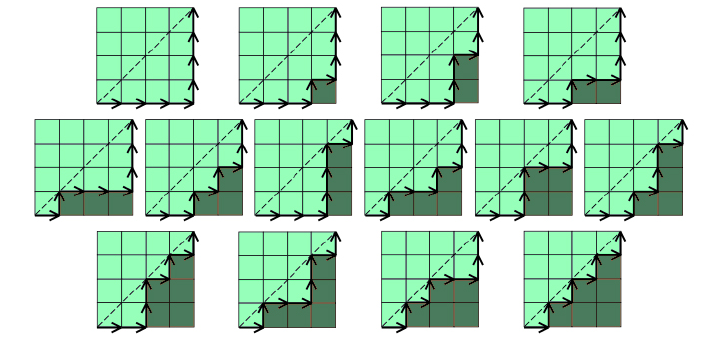
\includegraphics[width=280pt,height=160pt]{slike/catalan-net.png}
 		\caption{Putevi dužine 8 za tablu dimenzija $4\times 4$.} \label{fig:catalan-n-4}
 	\end{figure}
 	\item Broj permutacija skupa $\{1, \ldots, n \}$ koji ne sadrže patern \texttt{123} (ili bilo koji drugi, dužine 3) su predstavljeni Katalanovim brojevima. Npr. za $n = 3$, sljedeće permutacije zadovoljavaju uslove: $132,
 	213, 231, 312$ i $321$.  Dakle, ima ih ukupno 5. 
 \end{itemize}
 
 Prvih nekoliko Katalanovih brojeva su: $1, 1, 2, 5, 14, 42, 132,
 429, 1430, 4862, \ldots $
 
 
 Može se pokazati da za Katalanove brojeve vrijedi sljedeća rekurzija
 
 $$C(0) = 1, C(n+1) = \sum_{i=0}^{n} C(i) \cdot C(n-i), n \geq  0.$$
 
 Primijenimo metod brutalne sile (rekurzivno) pri računanju $n$-tog Katalanovog broja. Implementacija ovog pristupa je data sljedećim k\^odom. 
 
 \begin{minted}{python}
   def catalan(n):
       if n == 0:
          return 1
       catalan_n = 0 
       for i in range(n): 
           catalan_n += catalan(i) * catalan(n-1-i) 
       return catalan_n
        
 \end{minted}
  
  \emph{Kompleksnost algoritma}. Faktor grananja rekurzije je (najviše) $n$. Dubina rekurzije je $n+1$. Dakle, kompleksnost ovog algoritma je ogromna (eksponencijalna) i iznosi $O(n^n)$. 

Pokušajmo optimizovati ovaj (direktni) rekurzivni pristup. Iskoristimo princip memoizacije, zbog toga što se svaki podproblem izražunava iznova više puta. U nizovnoj strukturi $Cat(i)$ čuvajmo vrijednost $i$-tog Katalanovog broja prvi put kada se izračuna.  Vrijedi svojstvo optimalne podstrukture: $Cat(n+1) = \sum_{i=0}^{n} Cat(i) \cdot Cat(n-i).$ Bazni slučaj je dat sa $Cat(0) =1$.

Implementacija memoizacije je data sljedećim k\^odom.

  \begin{minted}{python}
	
	def initialization(n):
	   Cat = [ -1   for _ in range(n+1)  ] 
	   Cat[0]=1
	   return Cat 
	
	def catalan_i(i, Cat): 
	
	    if Cat[i] != -1:
	        return Cat[i]
     
            catalan_i = 0
            for k in range(i): 
                catalan_i += catalan_memoization(k, Cat) *
                     catalan_memoization(i-1-k, Cat)
    
            Cat[i] = catalan_i
            return Cat[i]
    
	   
	#poziv metode:
	n = 10
	Cat = initialization(n) 
	
	cat_n = catalan_n(n, Cat) 
	print(cat_n)
	
\end{minted}  

\emph{Kompleksnost algoritma}. Dubina rekurzije je (najviše) $n+1$. U svakoj rekurziji, broj iteracija koji se izvršava je linearne kompleksnosti $O(n)$. Prema tome, kompleksnost algoritma je $O(n) \cdot O(n) = O(n^2)$. 


 % sretni brojevi, semi-prosti brojevi... 
 
 %Lucky numbers... 
 Posmatrajmo konstrukciju niza brojeva opisanu sljedećom (iterativnom) procedurom.
 
 \begin{itemize}
 	\item Neka je dat niz brojeva:
 	$$1, 2, 3, 4, 5, 6, 7, 8, 9, 10, 11, 12, 13, 14, 15, 16, 17, 18, 19,\ldots $$
 	\item Izbrišemo svaki drugi broj iz skupa, čime dobijamo niz brojeva:
 	$$1, 3, 5, 7, 9, 11, 13, 15, 17, 19,\ldots$$
 	\item Iz prethodnog niza potom izbrišemo svaki treći broj, čime dobijamo novi niz brojeva: $1, 3, 7, 9, 13, 15, 19,\ldots$
 	\item Nastavljamo proceduru brisanja brojeva iz prethodnog niza tako što brišemo svaki četvrti broj u nizu itd.
 \end{itemize} 
 
 U ulazu se zadaje broj $n$. Ispitati da li je on \emph{srećan}, tj. da li neće biti obrisan prethodnom (iterativnom) konstrukcijom. 
 
 \begin{solution}
U prvoj iteraciji ($i=1$) će biti obrisani svi brojevi na parnoj poziciji u nizu, tj. oni koji su djeljivi sa $i+1=2$. Ako $n$ nije djeljiv sa $2$, preživjeće u ovoj iteraciji, te će se u novom (filtriranom) nizu pojaviti na poziciji $\lceil n/2 \rceil$. Dalje, u narednoj iteraciji ($i=2$) provjerimo da li je $\lceil n/2 \rceil < i+1=3$. Ako je to slučaj, broj $n$ nikad neće biti obrisan u narednim iteracijima, pa prekidamo pretragu, vraćajući rezultat \emph{True}. Inače, brišemo sve elemente novog niza čija je pozicija djeljiva sa $3=i+1$. Ako je $\lceil n/2 \rceil$ djeljiv sa 3, $n$ će biti obrisan (prekidamo pretragu, vraćajući rezultat \emph{False}). Inače, broj $n$ preživljava u ovoj iteraciji, te će se nakon operacije brisanja, pojaviti na poziciji $\lceil n/2 \rceil - \lceil n/2 /(i+1)\rceil = \lceil n/(i+1) \rceil = \lceil n/3 \rceil$ novonastalog niza. U narednoj iteraciji ($i=3$), sličnim rezonovanjem prvo provjeravamo da li je $\lceil n/3 \rceil < i+1=4$, pa vraćamo rezultat \emph{True}, ukoliko je to slučaj. Potom, provjeravamo da li je
 $\lceil n/3 \rceil$ djeljiv sa 4. Ako jeste, prekidamo pretragu i vraćamo rezultat \emph{False}. U protivnom, iz trenutnog niza brišemo sve elemente čija je pozicija djeljiva sa $4$, pa će se broj $n$ naći na poziciji $\lceil n/4 \rceil$ novonastalog niza. Ovaj proces ponavljamo, za svaku iteraciju, do prekida (u najgorem slučaju gornja granica broja iteracija je $n$).  
 
 
 Implementacija algoritma je data narednim k\^odom. 
 
 \begin{minted}{python}
 	from math import ceil
 	def lucky_number(n):
 
 	      
 	   for i in range(1, n): #iteracije
 	       if i+1 > ceil(n/i):
 	          return True 
 	       if ceil(n/i)  % (i+1) == 0:
 	          return False
 	   return True       
    
          #poziv funkcije
          print(lucky_number(7)) #True	       
  
 \end{minted}
  
 \end{solution}
 
 \section{Hornerov metod}
 %https://www.geeksforgeeks.org/mathematical-algorithms/
 %https://www.geeksforgeeks.org/horners-method-polynomial-evaluation/
\begin{definition}
	\textbf{\textit{Hornerov metod za računanje vrijednosti polinoma}}. Neka je dat polinom $P(x)=c_n x^n + c_{n-1}x^{n-1} + \cdots + c_1 x + c_0$ kao i tačka $x \in \mathbb{R}$. Naći vrijednost polinoma $P$ u tački $x$. Napomenimo da je ulaz vezan za polinom dat u obliku niza $ coef$ gdje   $coef[i]$ p˙redstavlja koeficijent uz monom  $x^{n-i}$, $i \in \{0, \ldots, n\}$. 

\end{definition}

\begin{solution}
	Pogledajmo primjer sljedeće instance: $coef = [1, -3, 2, -1], x = 3$. U ovom slučaju, riječ je o polinomu $P(x) =  x^3 - 3 x^2 + 2 x -1$. Izlaz    je $ P(3) = 5$.  \\
	
	Naivnim metodom, dakle računanjem vrijednosti $x^n$ običnom petljom se izvršava se u linearnoj $O(n)$ kompleksnosti. Kako imamo $n$ takvih vrijednosti za računanje (koji se potom sabiraju), ukupna kompleksnost ovakvog (naivnog) pristupa je $O(n^2)$.
	
	 Hornerovim metodom, računanje vrijednosti polinoma se može izvršiti u linearnoj $O(n)$ kompleksnosti. Ideju algoritma demonstrirajmo na primjeru polinoma iz prethodnog primjera, koji se može napisati kao:  $$((x - 3)x + 2)x -1.$$ 
	 Dakle, u tom slučaju, evaluacija ovako napisanog polinoma bi išla: prvo krećemo od koeficijenta $c_3=1$ kojeg množimo sa $x=3$ -- pri tome dobijamo (kumulativnu) vrijednost 3. Dalje, trenutnoj vrijednosti   dodajemo vrijednost narednog koeficijenta $c_2 = -3$, te dobijamo vrijednost 0, koju množimo sa $x=3$, dobijajući opet 0. Ponavljamo korak sa narednim koeficijentom $c_1 = 2$, čime dobijamo vrijednost 2, koju množimo sa $x=3$, dobijajući 6. Nadalje, posljednji koeficijent $c_0=-1$ jednostavno dodamo kumulativnoj vrijednosti, odakle dobijamo konačan rezultat, a to je 5. 
	 
	 Gledajući uopšteno, vrijedi: 
	 $$ c_n x^n + c_{n-1}x^{n-1} + \cdots + c_1 x + c_0 = ((\cdots ((c_n x + c_{n-1})x + c_{n-2})x + \cdots c_1) x + c_0  )$$
	 Trivijalni slučaj je  $n=0$, kada je $P(x) = c_0$. U tom slučaju, jednostavno vratimo vrijednost $ c_0$.
	 
	  
	 Implementacija algoritma Hornerovog metoda je data narednim k\^odom. 
	 
	 \begin{minted}{python}
	 	 def horner_metod(coef, n, x):
	 	    
	 	    if n == 0: 
	 	       return coef[0]
	 	    
	 	 	# inicijalizacija
	 	 	res = coef[n]  * x
	 	 	for i in range(1, n):
	 	     	res = res + coef[i]
	 	     	if i < n-1:
	 	     		res *= x
	 	 	return res
	 	 
	 	 # poziv funkcije
	 	 # Evaluacija:  x^3 - 3 x^2 + 2 x -1, x = 3
	 	 coef = [1, -3, 2, -1]
	 	 x = 3
	 	 n = len(coef)
	 	 print(horner_metod(coef, n, x))
	 \end{minted}

\textit{Kompleksnost algoritma.}  Jasno je da je najintenzivniji dio izvršavanja operacija smješten u \texttt{for}-petlju. Svaka iteracija se izvršava u konstantnom vremenu, pa zaključujemo da se algoritam izvršava u linearnom vremenu, tj. $O(n)$.  
\end{solution}
 
 %https://www.geeksforgeeks.org/sieve-of-atkin/ ==> SIEVE OF ATKIN ==> ako bude trebalo dodati...
 
 \section{Zadaci}
 
 \begin{enumerate}
 	\item Broj je poluprost (eng. \textit{semiprime}) ako se može predstaviti
 	kao proizvod dva (ne obavezno različita) prosta broja. Npr. $4, 6, 9, 10, \ldots$ su neki od poluprostih brojeva. Konstruisati (efikasan) algoritam koji ispituje da li je broj poluprost.
 	\item Broj je savršen akko je jednak zbiru svojih djelilaca (ne računajući njega samog). Npr. 6 i 28 su savršeni jer je $6 = 1 + 2 + 3; 28 = 1 + 2 + 4 + 7 + 14$. Napisati program koji ispituje da li je broj savršen korištenjem Eratostenovog sita. Kolika je vremenska složenost algoritma? Uporediti ovaj algoritam sa algoritamskom paradigmom brutalne sile.
 	\item Broj je ružan akko su mu jedini prosti faktori 2 ili 3 ili 5. Niz prvih ružnih brojeva je dat sa $1, 2, 3, 4, 5, 6, 8, 9, 10, 12, 15, \ldots$ (1 je po
 	konvenciji uključen). U ulazu je  dat broj $n$. Izračunati $n$-ti ružni broj. Koristiti paradigmu dinamičkog programiranja.
 	\item Sfenički brojevi su pozitivni cijeli brojevi koji se dobijaju kao proizvod tačno 3 različita prosta faktora. Npr. $30, 42, 66, 70, 78, 102, 105, 110, 114, \ldots$ su neki od takvih brojeva. U ulazu je dat broj $n$. Ispitati da li je on sfenički? 
 	
 	\textit{Primjer}. $30=2 \cdot 3 \cdot 5$ jeste sfenički, dok $60 = 2^2 \cdot 3 \cdot 5 $ nije sfenički. 
 	\item Za broj se kaže da je slobodan od kvadrata ako ga nijedan
 	prosti faktor ne dijeli više od jednom, tj. najveći stepen prostog
 	faktora koji dijeli $n$  je jedan.  Prvih nekoliko slobodnih kvadrata brojeva su $$1, 2, 3, 5, 6, 7,
 	10, 11, 13, 14, 15, 17, 19, 21.$$   Na ulazu je dat broj $n$. Ispitati da li je on broj 	slobodnog kvadrata.
 	\item Neka je dat broj $n$. Ispitati da li je to \textit{lažni} broj ili ne.
 	Pod lažnim brojem podrazumijevamo složeni broj, čiji je zbir cifara jednak zbiru cifara njegovih različitih prostih faktora.%https://www.geeksforgeeks.org/hoax-number/
 	
 	\item Dat je skup od $n$ elemenata, pronaći broj načina da se on particioniše (Belovi brojevi). Implementirati efikasnu proceduru računanja ovakvih brojeva u zavisnosti od $n$.  %https://www.geeksforgeeks.org/bell-numbers-number-of-ways-to-partition-a-set/
 \end{enumerate}